\chapter{Volume, Diagnosis, and the Hard Questions of Sales}

This chapter follows a School of Hard Knocks interview with Jacob Hopkins as a compact case study in early sales discipline, curated by LazyingArt LLC with Video2Book. Jacob is introduced as a nineteen-year-old college dropout who had taken on more than \(\$10{,}000\) in debt and later reached more than \(\$250{,}000\) per year in sales. We should read the interview neither as a guaranteed path nor as loose motivation. Its useful content is the sequence of mechanisms: repeated attempts reduce dependence on luck, listening turns a pitch into diagnosis, challenge tests whether a prospect's plan matches the prospect's goal, and hard questions make the close more responsible.

\section{The Opening Case And The Long Horizon}

James opens by naming the cast and the reason for the visit: he and Josh are there to talk with Jacob Hopkins about sales in the current market. The first quantitative frame is the credibility frame:

\begin{equation}
D > \$10{,}000,
\qquad
I_{\mathrm{sales}} > \$250{,}000/\mathrm{year}.
\end{equation}

Here \(D\) denotes the debt level reported in the introduction, and \(I_{\mathrm{sales}}\) denotes the reported annual sales income. These are interview claims, so they should be treated as source claims rather than audited financial facts. But they have a clear narrative role: before any tip is offered, the listener is told that the advice comes from a large change in circumstance.

Before Jacob gives his own five sales tips, the interview briefly turns to Quinn Fulmer, who describes the content side of acquisition.com. Quinn's point is about creators rather than closers: short form can bring people in the door, but copying other people and building a fast audience on a false foundation will not last. He frames the work as a three-, five-, or ten-year game. That aside is not accidental filler. It introduces the first durable theme of the chapter: a tactic is only as good as the longer path it serves.

\section{From Experiments To A Monetizable Skill}

Jacob's personal account begins with restlessness. In high school he was already looking for the next business. He did not want college in the ordinary sense, because he did not feel it fit the freedom he wanted. He tried car detailing, dropshipping, and real estate. Some of these attempts made a little money; none of them became the major engine.

The movement is important. Jacob does not begin with a polished doctrine of sales. He begins with experiments and with the discovery that a missing skill can make an otherwise promising business leak money. The narrative sequence is better represented as

\begin{equation}
\hbox{experiments}
\longrightarrow
\hbox{pressure}
\longrightarrow
\hbox{missing skill}
\longrightarrow
\hbox{sales career}.
\end{equation}

This is the first entrepreneurial lesson of the interview. A business idea may reveal the skill one lacks. In Jacob's account, sales becomes not an isolated job but the skill that makes commercial ambition operational.

The host then gives the interview its explicit structure: the point is to collect five sales tips for someone just starting out. The conversation moves from biography into operating rules.

\section{Volume Negates Luck}

Jacob's first rule is blunt: volume negates luck. He grounds it in the real estate period, where he says he was losing three or four thousand dollars per month:

\begin{equation}
L \approx \$3{,}000\hbox{--}\$4{,}000/\mathrm{month}.
\end{equation}

The advice he reports receiving was equally direct: if everyone else is making \(100\) calls, make \(200\). Jacob then says he made \(200\), \(300\), and \(400\) dials a day while others were making about \(100\):

\begin{equation}
N_{\mathrm{others}} \approx 100\ \mathrm{calls/day},
\qquad
N_{\mathrm{Jacob}} \approx 200\hbox{--}400\ \mathrm{dials/day}.
\end{equation}

We can express the mechanism cautiously. Let \(N\) be the number of qualified attempts in a period, and let \(p\) be the probability that a qualified attempt eventually produces a close. The transcript does not give \(p\), and real sales attempts are not identical independent trials. Still, as a first-order model,

\begin{equation}
\mathbb{E}[\hbox{closed deals}] \approx Np.
\end{equation}

Under that simplifying assumption, moving from \(100\) attempts to \(200\) attempts gives

\begin{align}
\frac{\mathbb{E}[\hbox{deals at }200]}{\mathbb{E}[\hbox{deals at }100]}
&\approx
\frac{200p}{100p} \\
&= 2.
\end{align}

This is not a proof that sales is only arithmetic. It is the disciplined core of Jacob's point. If a single call contains noise, then a larger number of serious repetitions produces more feedback, more chances to correct, and less dependence on one lucky conversation. Jacob says that within two or three weeks he was doing about as well as the others because he was simply putting up more numbers.

\subsection{Question \& Answer}

\paragraph{Question.}
If sales outcomes feel random, what can the beginner actually control?

\paragraph{Answer.}
The beginner controls the number of serious attempts and the rate of learning from them. Volume does not replace skill; it creates enough contact with reality for skill to form. One noisy call teaches little by itself. A day of repeated calls begins to show patterns.

\begin{figure}
\centering
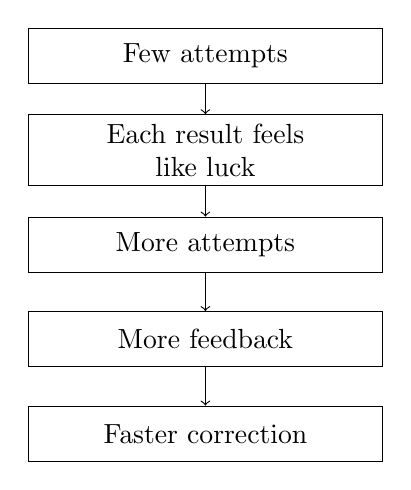
\begin{tikzpicture}[x=1cm,y=1cm]
\node[draw, align=center, minimum width=4.5cm, minimum height=0.7cm] (a) at (0,0) {Few attempts};
\node[draw, align=center, minimum width=4.5cm, minimum height=0.7cm] (b) at (0,-1.2) {Each result feels\\like luck};
\node[draw, align=center, minimum width=4.5cm, minimum height=0.7cm] (c) at (0,-2.4) {More attempts};
\node[draw, align=center, minimum width=4.5cm, minimum height=0.7cm] (d) at (0,-3.6) {More feedback};
\node[draw, align=center, minimum width=4.5cm, minimum height=0.7cm] (e) at (0,-4.8) {Faster correction};
\draw[->] (a) -- (b);
\draw[->] (b) -- (c);
\draw[->] (c) -- (d);
\draw[->] (d) -- (e);
\end{tikzpicture}
\caption{The first mechanism: volume turns isolated outcomes into repeated feedback.}
\end{figure}

\section{Performance Means Health Plus Action}

The interviewer next asks how someone maintains high performance in sales. This question matters because the first tip creates a cost. If the answer is more calls, then the seller has to remain able to make those calls.

Jacob's answer has two parts. First, take care of health: sleep and the ordinary physical conditions that make work repeatable. Second, act. He says that for him the biggest source of stress is inaction. If he is not hitting the phones or doing what he knows he needs to do, he gets stressed.

The distinction is not a psychological equation, but it can be written as a practical replacement rule:

\begin{equation}
\hbox{attention on outcome}
\quad \longrightarrow \quad
\hbox{attention on daily action}.
\end{equation}

The outcome is a lagging variable. The action is the input. In Jacob's telling, a salesperson stays steadier by measuring the thing that can actually be done today.

\subsection{Question \& Answer}

\paragraph{Question.}
How can high performance be maintained without becoming trapped by the result?

\paragraph{Answer.}
By keeping the body capable and the day active. Sleep and health sustain the machine; calls, practice, and follow-through give the mind something concrete to do. Stress is not eliminated by wishing for a close. It is reduced by returning to controllable work.

\section{Listen More, Pitch Less}

The second sales tip is ``listen more, talk less.'' Jacob pushes against the beginner's image of sales as a talking job. Articulation matters, but the sale is not created by filling empty space. It is created by understanding what the person wants, what the person needs, and why the purchase matters to them.

That diagnosis compresses the pitch. Jacob says that when he pitches, it is less than a minute:

\begin{equation}
T_{\mathrm{pitch}} < 1\ \mathrm{minute}.
\end{equation}

The mechanism is sequential:

\begin{equation}
\hbox{listen}
\longrightarrow
\hbox{diagnose}
\longrightarrow
\hbox{customize}
\longrightarrow
\hbox{brief pitch}
\longrightarrow
\hbox{ask}.
\end{equation}

The point is not that shorter is always better in isolation. The point is that the pitch becomes short because the conversation before it has done real work. Jacob says he can name the few relevant things based on what the prospect has already said. The pitch is therefore not a generic performance. It is the conclusion of listening.

\section{Long Horizon, Skill Stacking, And Challenge}

The interview then asks what Jacob would tell his younger self. This reflective question brings back the theme introduced by Quinn: time horizon. Jacob says he once tried to become a millionaire in \(90\) days, but that a safer way to think about becoming wealthy is in terms of ten years and the skill sets required for that path:

\begin{equation}
T_{\mathrm{fantasy}} \approx 90\ \mathrm{days},
\qquad
T_{\mathrm{skill\ path}} \approx 10\ \mathrm{years}.
\end{equation}

The transcript is garbled around the phrase that appears to mean skill stacking, so we should keep the reconstruction modest: if the business one wants to build requires selling, then sales is one of the skills to acquire before the later business can work.

This reflection leads into tip number three: challenge people. Jacob distinguishes challenging a prospect from being hostile. A salesperson is not merely the prospect's friend. The salesperson is trying to understand enough to test whether the prospect's beliefs and plans are consistent with the outcome the prospect says they want.

\subsection{Question \& Answer}

\paragraph{Question.}
How can a salesperson challenge a prospect without becoming adversarial?

\paragraph{Answer.}
The challenge must be anchored in the prospect's own goal. Jacob's example is a gym owner who wants to double membership in two years but says the plan is word of mouth. The salesperson does not attack the person. The salesperson asks whether the stated method can plausibly produce the stated result.

Jacob's concrete challenge is whether word of mouth can add \(300\) members in two years:

\begin{equation}
\Delta M \approx 300\ \mathrm{members},
\qquad
T = 2\ \mathrm{years}.
\end{equation}

A note writer may translate that into a monthly burden, while being clear that Jacob does not explicitly compute it in the transcript:

\begin{align}
\frac{\Delta M}{T}
&=
\frac{300\ \mathrm{members}}{2\ \mathrm{years}} \\
&=
150\ \mathrm{members/year} \\
&\approx
12.5\ \mathrm{members/month}.
\end{align}

This is the arithmetic behind the challenge. The moment the target is expressed as a rate, the prospect has to compare the current method with the required pace.

\begin{figure}
\centering
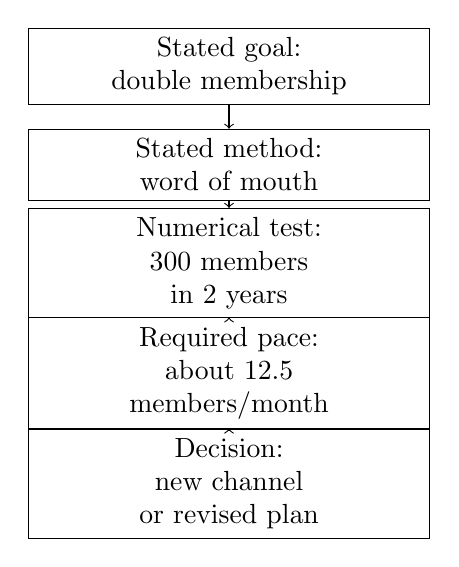
\begin{tikzpicture}[x=1cm,y=1cm]
\node[draw, align=center, minimum width=5.1cm, minimum height=0.72cm] (g) at (0,0) {Stated goal:\\double membership};
\node[draw, align=center, minimum width=5.1cm, minimum height=0.72cm] (m) at (0,-1.25) {Stated method:\\word of mouth};
\node[draw, align=center, minimum width=5.1cm, minimum height=0.72cm] (n) at (0,-2.5) {Numerical test:\\300 members\\in 2 years};
\node[draw, align=center, minimum width=5.1cm, minimum height=0.72cm] (r) at (0,-3.9) {Required pace:\\about 12.5\\members/month};
\node[draw, align=center, minimum width=5.1cm, minimum height=0.72cm] (d) at (0,-5.3) {Decision:\\new channel\\or revised plan};
\draw[->] (g) -- (m);
\draw[->] (m) -- (n);
\draw[->] (n) -- (r);
\draw[->] (r) -- (d);
\end{tikzpicture}
\caption{Challenge selling as a consistency test between goal, method, and required pace.}
\end{figure}

\section{Commission, Asking, And Referrals}

The next question raises a real obstacle for beginners: many sales roles are primarily commission based. Jacob does not deny that this is intimidating, and he does not claim it is for everyone. His answer is narrower. A salary is not absolute safety, because poor performance can still cost the job. Commission makes the performance link more direct.

A compact way to write the distinction is

\begin{equation}
\hbox{salary} \sim \hbox{indirect performance risk},
\qquad
\hbox{commission} \sim \hbox{direct performance exposure}.
\end{equation}

That is why Jacob calls sales close to owning a business. The seller has to manage time, schedule, effort, and output, and then gets paid according to production. The claim should not be stretched too far. A salesperson is not identical to an owner. But the role trains a narrow ownership-like discipline: results follow work more visibly.

Tip number four is then to ask for money. Jacob says too many people in sales do not actually ask for the order. The sequence is important: do not pitch until there is enough understanding to close, but once the pitch is made, ask.

He reports that people may say no five or ten times while he continues solving the problem and asking again:

\begin{equation}
n_{\mathrm{no}} \approx 5\hbox{--}10.
\end{equation}

In context, this should be read as persistence through objections, not as disregard for the prospect. The loop is

\begin{equation}
\hbox{objection}
\longrightarrow
\hbox{clarify}
\longrightarrow
\hbox{solve}
\longrightarrow
\hbox{ask again}.
\end{equation}

Networking and referrals extend the same pattern after the sale. Jacob describes clients seeing an ad, booking a call, joining the program, and then being asked whether they know anyone else who should be referred. He reports two closed deals in the previous week from that follow-up:

\begin{equation}
R_{\mathrm{closed}} = 2\ \mathrm{deals/week}
\end{equation}

for that reported week.

\subsection{Question \& Answer}

\paragraph{Question.}
Why does the interview treat commission as useful rather than merely risky?

\paragraph{Answer.}
Because it makes performance exposure explicit. Jacob's point is not that guaranteed income is bad or that commission suits everyone. It is that a person who wants to become entrepreneurial can learn from a role where effort, schedule, skill, and pay are tightly coupled.

\section{Stress And Hard Questions}

The interview returns to stress near the end. Jacob first normalizes it: stress can appear even when one is doing well, because the next uncertainty is always present. The first move is to register stress as a feeling rather than treat it as proof that something is wrong.

The second move is action. Jacob says to do more useful work: watch more game tape, listen to more sales calls, and take action. In his language, more action leaves less room for boredom, and boredom makes stress worse.

The fifth sales tip is that closers ask hard questions. Jacob gives examples: how much money is in the prospect's bank account, what happens if the problem is not fixed, what life looks like in five years without solving it, and what it looks like if the desired result does happen. These questions are awkward at first. The interview keeps that awkwardness visible because it is part of the skill.

\subsection{Question \& Answer}

\paragraph{Question.}
Why should a salesperson ask questions that feel uncomfortable?

\paragraph{Answer.}
Because the seller cannot responsibly recommend a program without knowing whether the prospect can succeed with it. Jacob says he cannot sign someone up if they do not have enough money to be successful. The hard question is therefore not decoration and not mere pressure. It is part of diagnosis.

The whole interview can be summarized as a control loop:

\begin{figure}
\centering
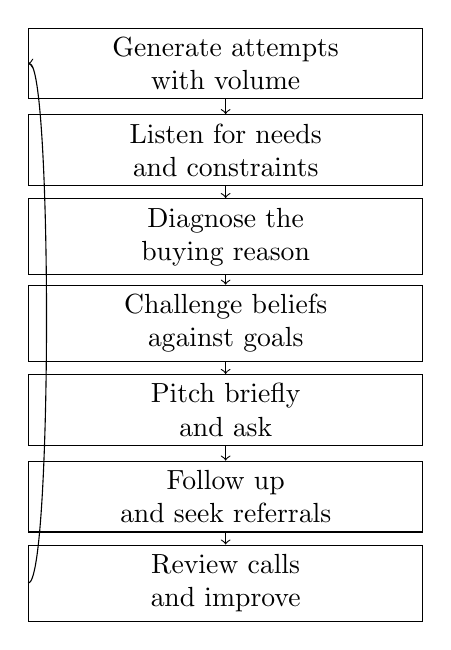
\begin{tikzpicture}[x=1cm,y=1cm]
\node[draw, align=center, minimum width=5.0cm, minimum height=0.66cm] (a) at (0,0) {Generate attempts\\with volume};
\node[draw, align=center, minimum width=5.0cm, minimum height=0.66cm] (b) at (0,-1.1) {Listen for needs\\and constraints};
\node[draw, align=center, minimum width=5.0cm, minimum height=0.66cm] (c) at (0,-2.2) {Diagnose the\\buying reason};
\node[draw, align=center, minimum width=5.0cm, minimum height=0.66cm] (d) at (0,-3.3) {Challenge beliefs\\against goals};
\node[draw, align=center, minimum width=5.0cm, minimum height=0.66cm] (e) at (0,-4.4) {Pitch briefly\\and ask};
\node[draw, align=center, minimum width=5.0cm, minimum height=0.66cm] (f) at (0,-5.5) {Follow up\\and seek referrals};
\node[draw, align=center, minimum width=5.0cm, minimum height=0.66cm] (h) at (0,-6.6) {Review calls\\and improve};
\draw[->] (a) -- (b);
\draw[->] (b) -- (c);
\draw[->] (c) -- (d);
\draw[->] (d) -- (e);
\draw[->] (e) -- (f);
\draw[->] (f) -- (h);
\draw[->] (h.west) .. controls (-2.2,-6.6) and (-2.2,0) .. (a.west);
\end{tikzpicture}
\caption{The sales control loop reconstructed from the five tips.}
\end{figure}

\section{Summary}

The interview unfolds from case to mechanism. First we are given Jacob's reported transformation, then his early business experiments, and only then the sales rules. That order matters. The tips are not floating slogans; they answer specific pressures: uncertainty, performance cost, poor listening, weak prospect beliefs, commission fear, reluctance to ask, beginner stress, and awkward questions.

The quantitative spine is modest but important. The chapter preserves the concrete figures that make the advice inspectable: more than \(\$10{,}000\) in reported debt, more than \(\$250{,}000\) per year in reported sales income, \(\$3{,}000\) to \(\$4{,}000\) in monthly real estate losses, \(100\) calls versus \(200\) to \(400\) daily dials, a two- to three-week catch-up claim, a pitch under one minute, \(300\) gym members over two years, five to ten refusals, and two referral deals in a week. The numbers do not make the interview scientific in the laboratory sense. They keep the commercial reasoning concrete: sales improves when effort, diagnosis, challenge, and asking become repeatable.